\documentclass[11pt]{article}

\usepackage[sort]{natbib}
\usepackage{fancyhdr}

% include other packages here (next line)
\usepackage{enumitem}
\usepackage{graphicx}
\graphicspath{ {images/} }

\usepackage{titlesec}

\titleformat{\section}
  {\normalfont\fontsize{11}{11}\bfseries}{\thesection}{1em}{}
\titlespacing\section{0pt}{11pt plus 4pt minus 2pt}{0pt plus 2pt minus 2pt}
\titlespacing\subsection{0pt}{11pt plus 4pt minus 2pt}{0pt plus 2pt minus 2pt}
\titlespacing\subsubsection{0pt}{11pt plus 4pt minus 2pt}{0pt plus 2pt minus 2pt}

\setlist[itemize]{noitemsep, topsep=0pt}

%----- page properties -----------------
\usepackage[margin=0.5in]{geometry}
%\oddsidemargin 0.2cm
\topmargin -1.0cm
\textheight 22.5cm
%\textwidth 15.25cm
\parindent=0pt
\parskip 1ex
\renewcommand{\baselinestretch}{1.1}
\pagestyle{fancy}
%----------------------------------------------------



% header and footer ----------------------------------

\lhead{\normalsize \textrm{ChBE 8803 Project (Group 13)}}
\chead{}
\rhead{\normalsize Milestone 02.02.18}
\lfoot{\normalsize \textrm{Rebecca Han}}
\cfoot{}
\rfoot{Jack Findley}
\setlength{\fboxrule}{4pt}\setlength{\fboxsep}{2ex}
\renewcommand{\headrulewidth}{0.4pt}
\renewcommand{\footrulewidth}{0.4pt}

    
\begin{document}


%----------------your title below -----------------------------

\begin{center}
{\bf Identifying Cell Nuclei in Divergent Images }
\end{center}

%---------------- start of document body------------------
\section{Background}

Pathologists use immunohistochemistry (IHC) to detect tumours by identifying and quantifying the presence of important biomarkers expressed in cell nuclei. However, manual identification is time-consuming, thus it is highly desirable to develop an automated, high-accuracy method for isolating and analyzing nuclei in different kinds of IHC images.

\section{Data Description \& Challenge}

The dataset is challenging because of high volume and dimensionality. Our data is divided into a training set (670 images, each containing between 1 to 100 masks for distinct nuclei) and test set (65 images). The images vary in size (total pixels) and were collected from many different cell types under a variety of imaging conditions (magnification, modality, etc). To achieve success, we will have to work with all the given data to develop a robust method for cell nucleus identification.

\section{Hypotheses \& Goals}

\textbf{\textit{Goal 0. One-index the pixels in each image from top to bottom, left to right.}}

\textbf{\textit{Goal 1. Normalize across set of images.}}\\
The variety of cell type, staining and imaging condition all complicate cell identification. Pre-processing the data will ensure comparison across uniform images.

\textbf{\textit{Goal 2. Identify all objects in each image.}}\\
We will separate objects from background, categorizing each pixel as ground or non-ground.

\textbf{\textit{Goal 3. Separate individual cell nuclei.}} Once we have distinguished all objects as distinct from ground, the next step is to determine individual cells. For each image, we will return a set of masks, each mask only covering one nucleus with no overlap between any of the masks.

\textbf{\textit{Goal 4. Maximize average precision.}}\\
Precision is the number of true positives divided by the sum of the number of true positives, false positives and false negatives. This is defined as a function of an intersection over union (IoU) threshold \textit{t} between a set of predicted pixels A and a set of true object pixels B. For each image, we want to maximize average precision for \textit{t} $\in$ [0.5, 0.55, 0.6, 0.65, 0.7, 0.75, 0.8, 0.85, 0.9, 0.95].

\section{Definition of Success}

Success is a defined as a workflow that consists of pre-processing to normalize variation in imaging condition, separating objects from background in each image, and distinguishing individual cell nuclei. The differences in low, expected and high success are based on model accuracy as follows.

\textbf{\textit{Low:}} Accomplish Goals 0-2. For Goal 3, predict nuclei regardless of accuracy.

\textbf{\textit{Expected:}} Accomplish Goals 0-3. For Goal 4, achieve 
\begin{itemize}
\item \textgreater 65\% accuracy for threshold values 0.5, 0.55, 0.6, 0.65
\item \textgreater 75\% accuracy for threshold values 0.7, 0.75, 0.8, 0.85
\item \textgreater 85\% accuracy for threshold values 0.9, 0.95
\end{itemize}

\textbf{\textit{High:}} Accomplish Goals 0-3. For Goal 4, achieve
\begin{itemize}
\item \textgreater 80\% accuracy for threshold values 0.5, 0.55, 0.6, 0.65, 0.7
\item \textgreater 90\% accuracy for threshold values 0.75, 0.8, 0.85, 0.9, 0.95
\end{itemize}

\section{Deliverables}

The key deliverable will be a Jupyter notebook containing:

\begin{itemize}
\item Code to convert images to one-indexed pixels and normalize the data from different imaging conditions
\item Code to separate objects from the background
\item Code to identify individual nuclei
\item Documentation of the inputs and outputs of all functions
\item Quantitative assessment of model accuracy
\item Written critical analysis of successes/failures of the model
\end{itemize}

\section{Schematic}

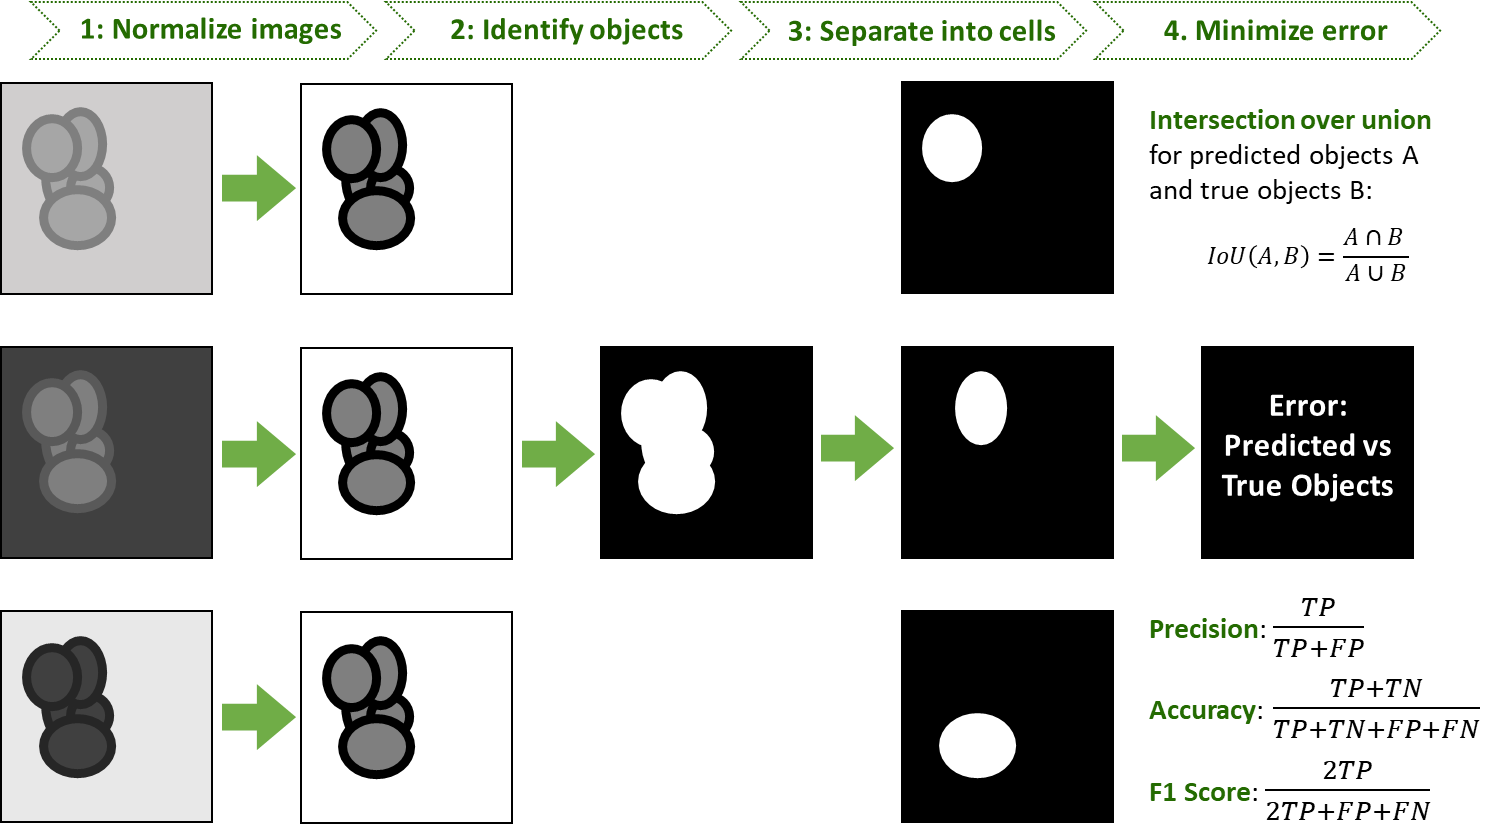
\includegraphics[width=19cm]{schematic}


%\hspace*{1em} Mathematical modelling through differential equations have a large number of real world applications, such as population growth. Outside of a handful of systems we do not have exact solutions to these differential equations. Therefore, it falls to either approximations or numerical methods. Numerical methods are used to solve intial value problems or boundary value problems and all of these methods involve discretisation (i.e. continuous functions on the interval $[a,b]$ of x replaced by points $x_{n}=a+nh$ where $n=0,1,2,...N$ and $h$=stepsize).\\
%``An intial boundary value problem can be defined as 
%\begin{equation}
%\frac{dy}{dx}=f(t,y),
%\end{equation}
%for $a\leq t\leq b$ subject to an intial condition; $y(a)=\alpha$."  \citep{Faires}\\
%\hspace*{1em}    More precisely, numerical methods is a differance equation including a number of consecutive approximations ($y_{n+j},j=0,1,...,k$). We can therefore compute, by sequential methods, the sequence {$y_{n}|n=0,1,2,...,N$}; natuarally this differance equation involves the function $f$. The integer $k$ is called the \textit{stepnumber} of the method; if $k=1$, the method is known as a \textit{one-step} method. \citep{Lambert1991}\\
%\hspace*{1em}    At this point, it is important to state that for this project it is sufficient to only cover explicit numerical methods. So, in other words $y_{n+j}$ is given in terms of previously computed values $y_{j}$, where $j\leq n$.\\
%\hspace*{1em}    The most basic \textit{one-step} explicit method is known as Euler's method, for now only showing the foward differance method is sufficient.
%\begin{equation}
%x_{n+1}-x_{n} = hf(t_{n},x_{n}), n=0,1,2,...N
%\end{equation}
%computing the sequence {$x_{n}$} given that $x_{0}=\alpha$. \citep{Griffiths}\\
%\hspace*{1em}    Euler's method is a good starting point but has its limitations, to increase accuracy (i.e. how far our approximations are from the exact solution) we either increase the order of Taylor expansion or find a better approximation. \textit{Multi-step} methods (i.e. if $k>1$, the method is called a \textit{multistep} or \textit{k-step} method)
%are now introduced as more accurate approximations. The Adams-Bashforth is a strongly recognized method for its accuracy and is the two step method associated with Euler's Rule as it is also explicit. It can be defined as
%\begin{equation}
%x_{n+2}-x_{n+1}=\frac{1}{2}h(3f_{n+1}-f_{n}),
%\end{equation} 
%
%where $f_{n}=f(t_{n},x_{n})$ and $f_{n+1}=f(t_{n+1},x_{n+1})$. \citep{Griffiths}\\
%\hspace*{1em}   The numerical methods have been establised and it is natural to progress into finding ways to test and compare which methods are best. \textbf{Accuracy} has already been mentioned, in detail it falls to define; \textit{local error}, \textit{global error} and \textit{truncation error}. \textbf{Convergance} follows from this, the aim being at each step of the method to converge to the exact solution as our stepsize ($h$) tends to zero. Lastly \textbf{stability} is desired, more specifically: \textit{zero}, \textit{aboslute} and \textit{relative} stability. Stability concerns itself with making sure small changes in our data to not cause large changes in the solution created by our method.\\
%\hspace*{1em}    In conlusion, we aim to find efficiency in these methods through rigorous testing.

























% ----------------end of document body---------------------

%---------------- start of references------------------

%\begin{thebibliography}{999}
%\bibitem[Faires \& Burden(1998)]{Faires}{Faires.D.J \& Burden.R. (1998). \textit{Numerical methods: second edition}. USA: Brooks/Cole Publishing Company}
%\bibitem[Griffiths \& Highams(2010)]{Griffiths}{Griffiths.D.F. \& Highams.D.J.(2010). \textit{Numerical methods for Ordinary Differential equations: Initial Value Problems}. London: Springer Undergraduate Mathematics series.}
%% ---Not currently cited but kept in for future referance----\bibitem[Lambert(1973)]{Lambert1973}{Lambert.J.D.(1973). \textit{Computation Methods in Ordinary Differential Equations}, New York: John Wiley \& Sons.}
%\bibitem[Lambert(1991)]{Lambert1991}{Lambert.J.D.(1991). \textit{Numerical Methods for Ordinary Differential Systems: The Initial Value Problem}, West Sussex: John Wiley \& Sons Ltd.}
%
%
%\end{thebibliography}

%---------------- end of references------------------


\end{document}